% yaml_vertical.tex
% Vertical flow diagram - optimized for single column width
% Shows the core transformation: YAML file → Stata frame → programmatic access
% Author: João Pedro Azevedo
% Date: December 2025

\documentclass[tikz,border=8pt]{standalone}
\usepackage{tikz}
\usetikzlibrary{positioning, arrows.meta, shapes.multipart}

\begin{document}

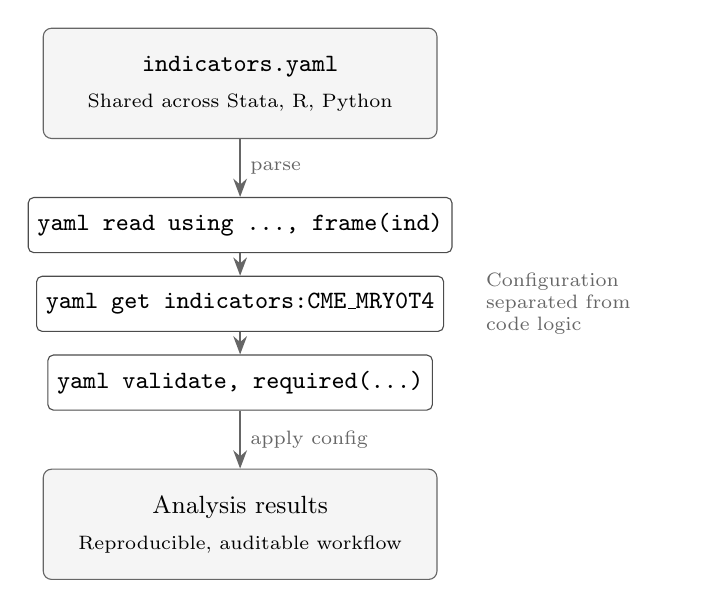
\begin{tikzpicture}[
    % Clean styles
    filebox/.style={
        rectangle, 
        rounded corners=3pt,
        draw=black!60, 
        fill=gray!8,
        minimum width=5cm, 
        minimum height=1.4cm,
        font=\small,
        align=center
    },
    cmdbox/.style={
        rectangle, 
        rounded corners=2pt,
        draw=black!70, 
        fill=white,
        minimum width=4cm,
        minimum height=0.7cm,
        font=\small\ttfamily
    },
    arrow/.style={
        ->,
        >=Stealth,
        thick,
        black!60
    },
    note/.style={
        font=\scriptsize,
        text=black!60
    }
]

% === Top: YAML Source ===
\node[filebox] (source) at (0, 4) {
    \texttt{indicators.yaml}\\[2pt]
    {\scriptsize Shared across Stata, R, Python}
};

% === Middle: Stata with yaml command ===
\node[cmdbox] (read) at (0, 2.2) {yaml read using ..., frame(ind)};
\node[cmdbox] (get) at (0, 1.2) {yaml get indicators:CME\_MRY0T4};
\node[cmdbox] (validate) at (0, 0.2) {yaml validate, required(...)};

% === Bottom: Output ===
\node[filebox] (output) at (0, -1.6) {
    Analysis results\\[2pt]
    {\scriptsize Reproducible, auditable workflow}
};

% === Arrows ===
\draw[arrow] (source) -- node[right, note] {parse} (read);
\draw[arrow] (read) -- (get);
\draw[arrow] (get) -- (validate);
\draw[arrow] (validate) -- node[right, note] {apply config} (output);

% === Side annotation ===
\node[note, anchor=west, text width=2.5cm, align=left] at (3, 1.2) 
    {Configuration\\separated from\\code logic};

\end{tikzpicture}

\end{document}
